\hypertarget{decision-theory}{%
\section{Decision Theory}\label{decision-theory}}

\begin{figure}
\centering
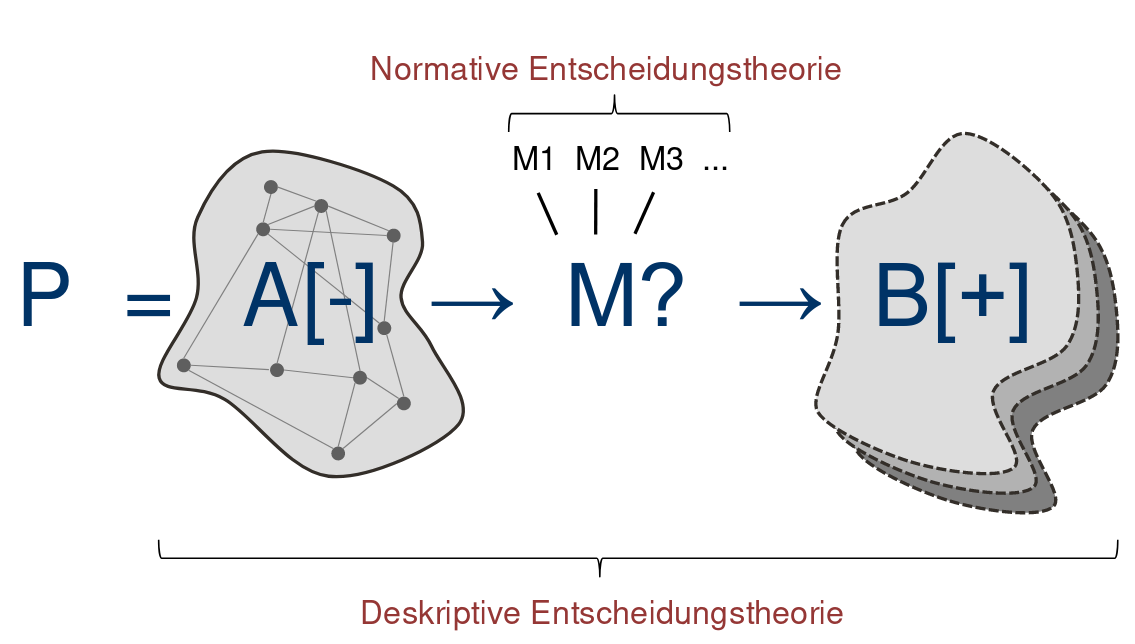
\includegraphics{figures/decisionTheory.png}
\caption{Decision Theory}
\end{figure}

There are two perspectives on the decision theory in this course. The
\textbf{descriptive decision theory} describes the way how the decisions
were made (already done).

The \textbf{normative decision theory} describes how the decisions
should be made. What options are available, what should be respected?

\hypertarget{decriptive-decision-theory}{%
\subsection{Decriptive Decision
Theory}\label{decriptive-decision-theory}}

\begin{itemize}
\tightlist
\item
  Intuitive and rational decisions
\item
  Mental models
\end{itemize}

\textbf{Rational decisions} are \textbf{targeted throughout} and
\textbf{goal oriented, based on objectiv informations}. They follow a
\textbf{systematic procedure} and \textbf{uses a clear methodological
rules} (which is understandable from not involved people). These
decisions are \textbf{not from gut feeling} and are \textbf{not
intuitiv}.

The fundamental of a \textbf{intuitive decision} is the
\textbf{knowledge} you have and \textbf{the experience of everything}
you ever experienced or of happenings and knowledge you earned from
other people. Decisions made out of \textbf{gut feeling}.

A \textbf{mental model} is a \textbf{simplified mental description of
the experienced world} with the purpose of - \textbf{handling the large
quantity of information} - in order to be able to \textbf{make decisions
quickly}

e.g.~If your coin doesn't get accepted in the vendor machine, you need
to rub it on the surface of the machine and try it again. And if this
works, it even strengthen your mental model, but actually this process
with the coin doesn't help in any way.

Second example: You try to cross the road and you are at the edge of the
sidewalk. If there are no noise, you are able to cross the road. But no
noise is actually not a proof that the street if safe to cross.

Mental models are \textbf{made of} - \textbf{Subconscious} - \textbf{By
experience} in the past - and they are adapted to specific situations
immediately

\begin{verbatim}
Learning is nothing else than adapting mental models.
If you are not able to adapt mental models, you are not able to make decisions quickly.
\end{verbatim}
